In this section, we present our approach to root cause diagnosis for Cloud VR applications as a time series classification problem. The dataset of $T$ multivariate time series KPIs is represented as $\mathcal{D}_{train} =  \{(w_1, y_1), (w_2, y_2) \ldots, (w_T, y_T)\}$ where $w_t \in \mathbb{R}^{p \times m}$ is a $p \times m$-dimensional vector corresponding to the KPIs values for time steps $t, t+1, \ldots, t+p-1$, and $y_t$ is a one-hot encoded label vector of size $K$. $\forall j \in [|1, K|]$, $j=1$ if $w_t$ belongs to class $j$ and $y_{t,j}$ 0 otherwise.

The task of root cause diagnosis is to learn a classification model $f_\theta$ on $\mathcal{D}_{train}$ that can assign the root cause $y_t$ for any newly observed time series $\tilde{w}_t$. To achieve this, we propose RAID, a two-stage architecture comprising i) an \textbf{anomaly detection stage} and ii) a \textbf{root cause classification stage}.


\subsection{Anomaly detection stage}
The anomaly detection stage identifies whether a time series is anomalous, using a self-supervised learning approach based on contrastive learning. This stage eliminates the need for labeled data by leveraging only normal data collected during Cloud VR sessions without Wi-Fi impairments.
%$\mathcal{D}_{normal} =\{w_1, \ldots, w_N\}$ 
Traditional anomaly detection methods rely on techniques such as reconstruction-based, isolation-based, one-class classification, or generative models, which detect anomalies by modeling the concept of normality and measuring deviations from it. While effective, these approaches often fail to capture nuanced temporal dependencies and complex patterns in time-series data. 

\begin{figure*}[!ht]
    \centering
    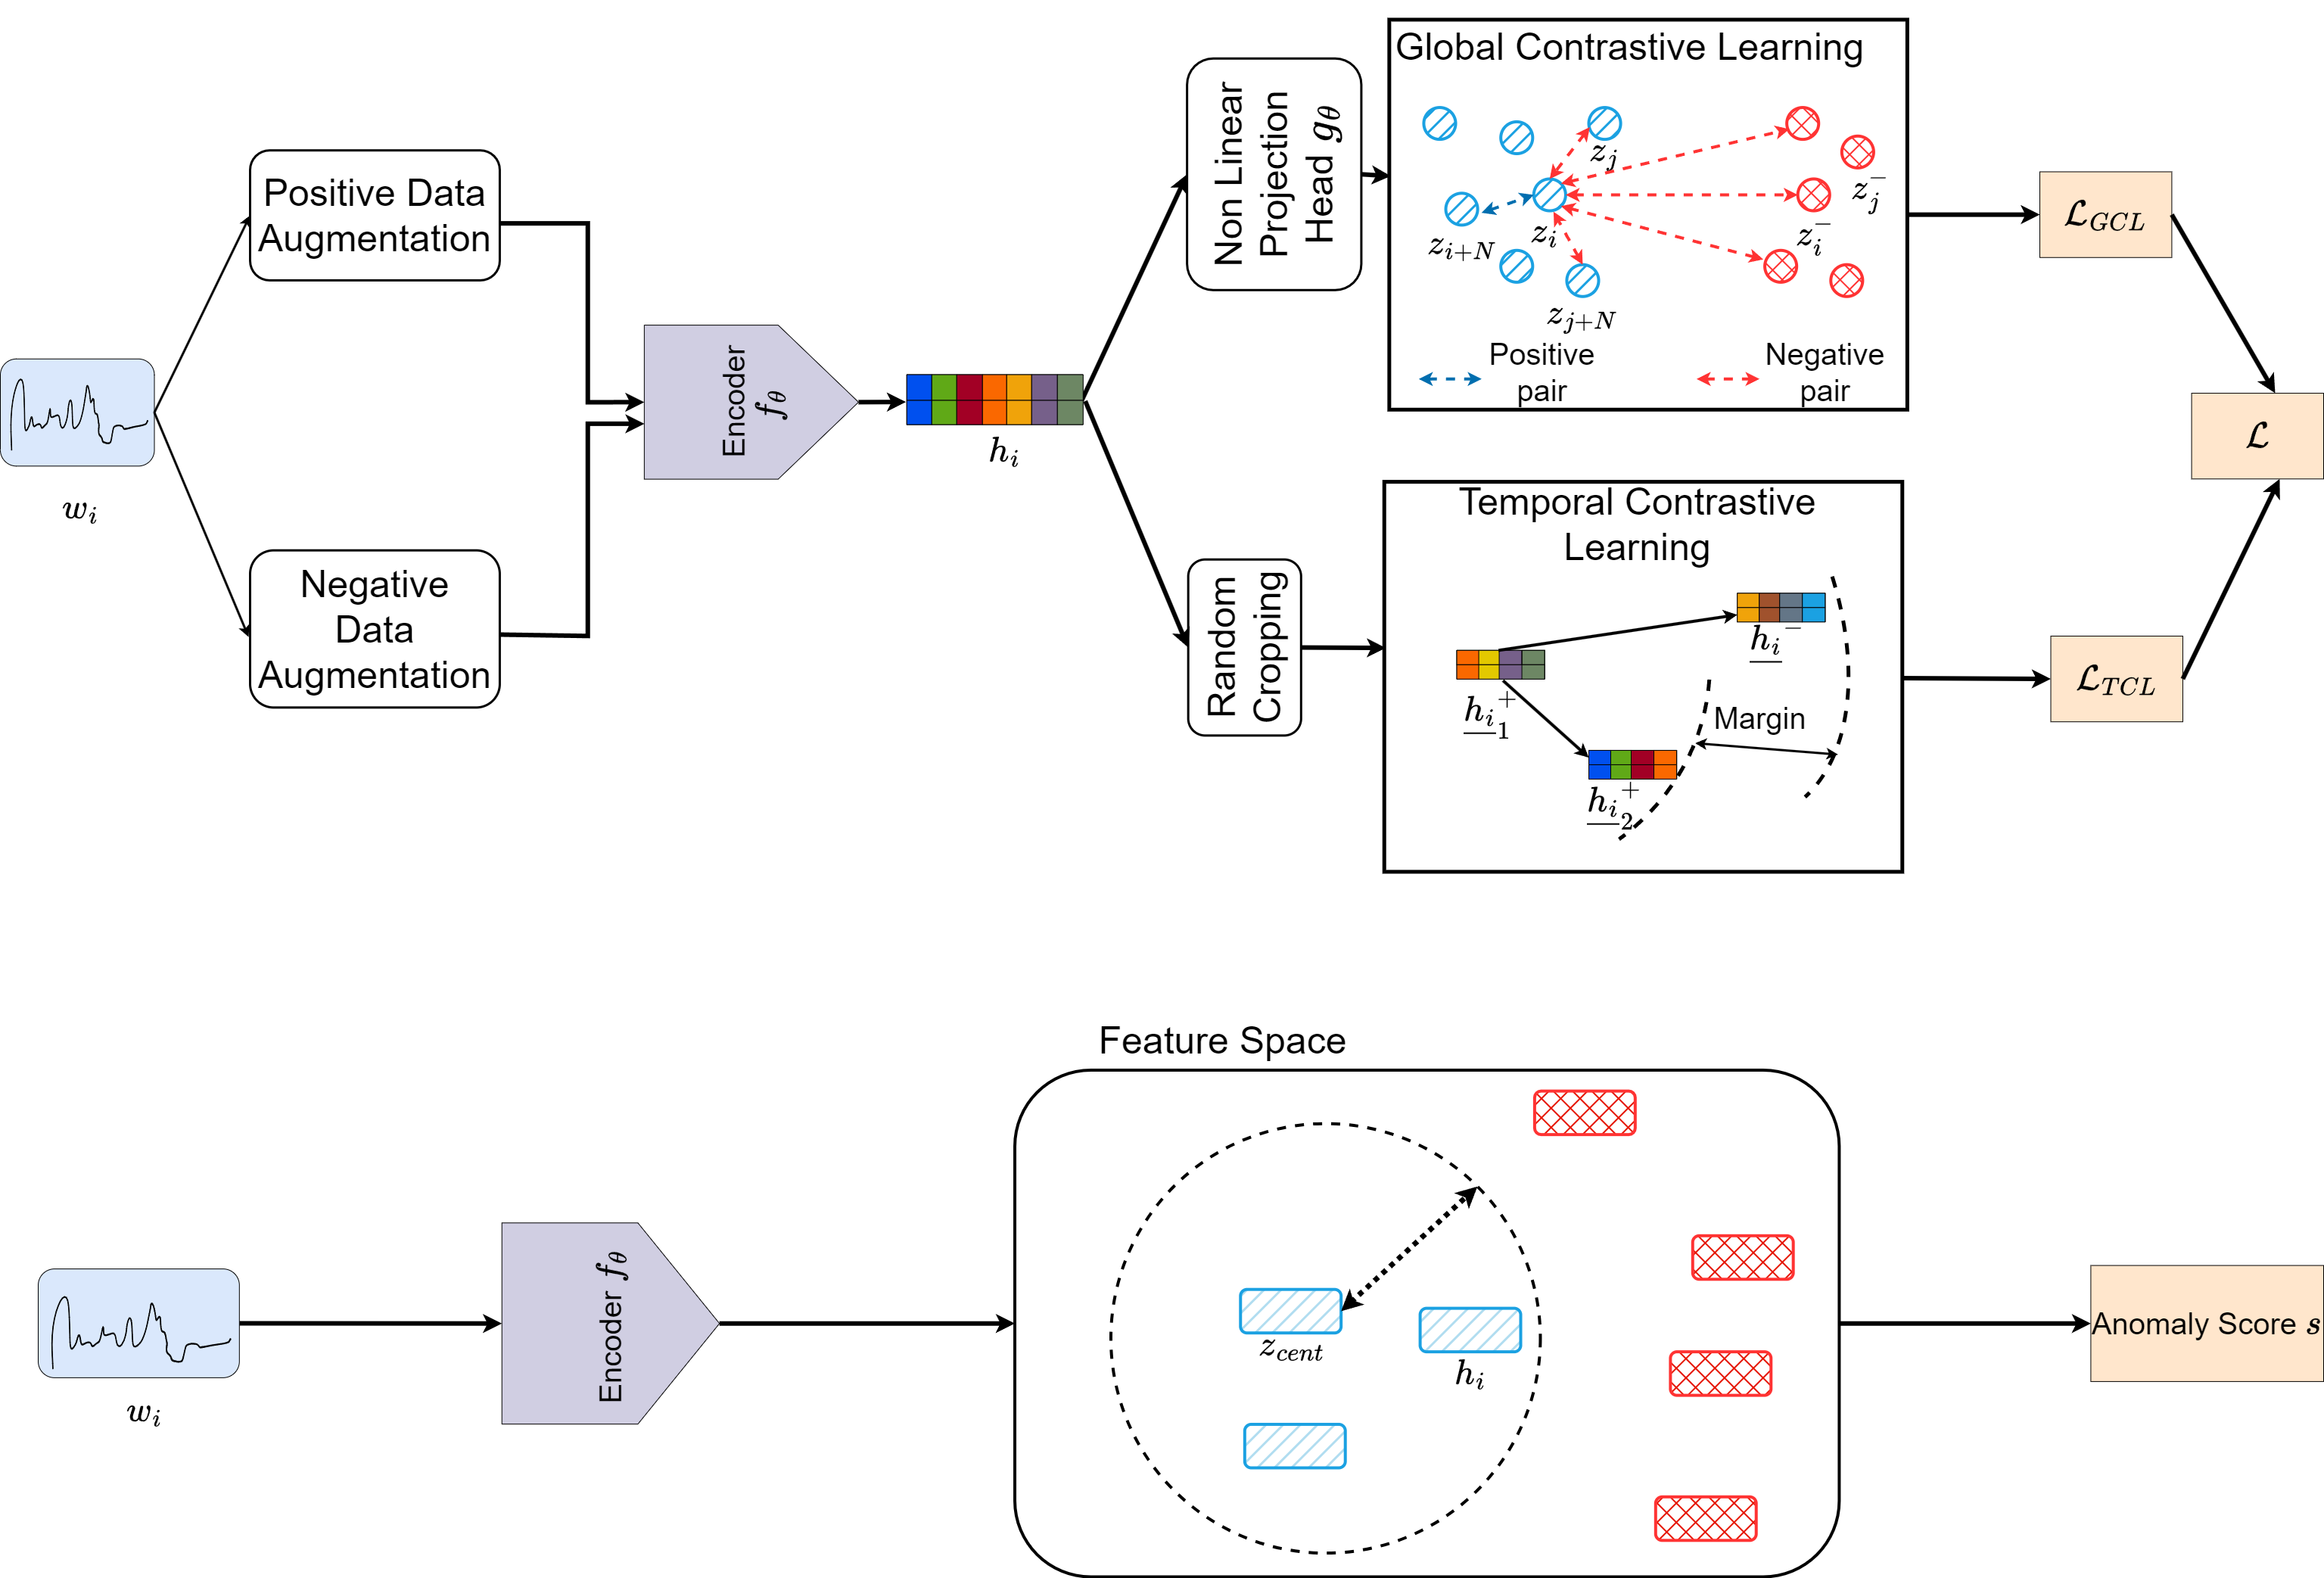
\includegraphics[width=\linewidth]{imgs/chapter_6/cats.png}
    \caption{Anomaly detector}
    \label{fig:chap_6:cats}
\end{figure*}

We adopt the CATS framework, summarized in Fig. \ref{fig:chap_6:cats}, described in Chapter \ref{chap:cats} which leverages temporal contrastive learning to learn robust representations of normal behavior. CATS enhances anomaly detection through synthetic anomaly generation and temporal contrastive loss formulations. The anomaly detector is trained using the loss combining global and temporal contrastive loss ($\frac{1}{2} (\mathcal{L}_{TCL} + \mathcal{L}_{GCL})$) and consists of the following components:
\begin{itemize}
    \item Data augmentation module. We generate views from time series: positive views using \textit{jitter} and \textit{scaling} to generate altered versions of normal data ensuring transformation-invariant representations. Synthetic anomalies are also generated using masking and trend transformations, bringing anomaly-related knowledge into the model.
    
    \item An encoder that encodes augmented time series into a low-dimensional latent space. The encoder is model-agnostic, allowing flexibility in its architecture (e.g., convolutional, recurrent, or transformer-based models).
    
    \item A projection head that maps the latent representations to a space optimized for contrastive learning. Typically implemented as a non-linear three-layer MLP \cite{chen2020simple}
    
    \item A temporal contrastive loss captures temporal similarity using a differentiable variant of DTW, Soft Dynamic Time Warping (Soft-DTW)-based triplet loss. This loss ensures that temporally similar representations are clustered while separating non-similar instances. This loss is defined as follows:
    \begin{equation}
        \mathcal{L}_{TCL} = \frac{1}{N} \sum_{i=1}^{N} max(D^{\gamma}(\underline{h_i}_1^+ - \underline{h_i}_2^+) - D^{\gamma}(\underline{h_i}_1^+ - \underline{h_i}^-) + m; 0)
    \end{equation}
    where $D^{\gamma}(.)$ is the Soft-DTW divergence measure, $m$ the margin parameter (minimum distance that must be kept between positive samples and negative samples).
    
    \item A global contrastive loss uses the Normalized Temperature-Scaled Cross-Entropy Loss (NT-Xent) to learn global feature similarities. This loss incorporates an expanded set of negative pairs to improve contrastive learning. \cite{chen2020simple}. This loss is defined as follows:
    \begin{equation}
        \mathcal{L}_{GCL} = \frac{1}{2N} \sum_{i \in \mathcal{B}^{+}} log \frac{exp(sim(z_i, z_{i+N})/\tau)}{\sum_{j \in \mathcal{B} \text{ and } j \neq i} exp(sim(z_i, z_j)/\tau)}
    \end{equation}
    with $\mathcal{B} = \mathcal{B}^{+} \cup \mathcal{B}^{-}$, $N$ the batch size, $\tau$ the temperature hyperparameter and $sim(.)$ the cosine similarity.
    
    \item Anomaly detection: After training, the encoder is retained to compute anomaly scores for unseen data. The score is the distance between the latent representation of the time series and the centroid of normal representations. An anomaly is flagged if the score exceeds a predefined threshold. The anomaly score is defined as follows:
    \begin{equation}
    \begin{split}
        s(\tilde{w_t}) &= \mathcal{D}(f_{\theta}(\tilde{w_t}), z_{cent}) \\
                       &=  \mathcal{D}(\tilde{z_t}, z_{cent}) \\
                       &=  \mathcal{D}(\tilde{z_t}, \frac{1}{N_{train}} \sum_{i=1}^{N_{train}} w_i) \\
    \end{split}
    \end{equation}
    where $\mathcal{D}$ is the Euclidean distance.
\end{itemize}

% \subsection{Root cause classification}
% Once an anomaly is detected, the next step is to determine its underlying root cause. This stage is framed as a supervised classification problem, where the objective is to map each detected anomaly to a predefined class of root causes $\{cause_1, cause_2, \ldots, cause_{K-1}\}$. To ensure efficiency and simplicity, we use a shallow classifier such as logistic Regression or Support Vector Machine (SVM) despite the various techniques for supervised TSC that were proposed in the literature. This approach, as showed in the following sections, achieves high accuracy with minimal computational overhead, making it suitable for real-time deployment.

\subsection{Root Cause Classification}

Once an anomaly is detected, the next step is to determine its underlying root cause. This stage is framed as a supervised classification problem, where the objective is to map each detected anomaly to a predefined class of root causes $\{cause_1, cause_2, \ldots, cause_{K-1}\}$.

To ensure efficiency and simplicity, we use a shallow classifier, a \ac{SVM}. Despite the numerous techniques for supervised TSC proposed in the literature, this model is efficient enough for our task given the anomaly detection stage previously executed. 

SVM are supervised learning algorithms designed to find the optimal hyperplane that separates data into distinct classes in a feature space. In the context of root cause classification, the input of time series flagged as anomalies ${(x_i, y_i)}_{i=1}^{N_{train}}$ are fed as input to the SVM classifier. The SVM employs a kernel trick (a kernel function $k$ satisfying $k(x_i, x_j) = \phi(x_i) \phi(x_j)$) to map inputs into a higher-dimensional space where a linear separation is possible. We use the \ac{RBF} kernel function ( $k(x_i, x_j) = \exp(-\gamma |x_i - x_j|^2)$). The classifier next identifies the hyperplane that maximizes the margin between the classes by solving the dual problem.

\begin{equation}
\begin{split}
    \min_{\alpha} & \quad \frac{1}{2} \sum_{i, j=1}^{N_{train}} \alpha_i \alpha_j y_i y_j k(x_i, x_j) - \sum_{i=1}^{N_{train}}  \alpha_i, \\
    \text{s.t} \quad & 0 \leq \alpha_i \leq C, \quad \forall i = 1, \ldots, N_{train} \\
                & \sum_{i=1}^{N_{train}}  \alpha_i y_i = 0
\end{split}
\end{equation}


where $\alpha_i$ are the Lagrange multipliers obtained by solving the dual optimization problem; $C > 0$ is the regularization parameter that controls the trade-off between maximizing the margin and minimizing classification errors; $y_i$ are the labels of the training data points and $x_i$ are the feature vectors of the training data.
% \begin{itemize}
%     % \item $w$ is the weight vector defining the orientation of the hyperplane.
%     % \item $b$ is the bias term determining the offset of the hyperplane from origin.
%     %\item $K(\mathbf{x}_i, \mathbf{x}_j)$ is the kernel function, defined as $K(\mathbf{x}_i, \mathbf{x}_j) = \phi(\mathbf{x}_i)^\top \phi(\mathbf{x}_j)$, which computes the dot product in the feature space induced by $\phi$.
%     \item $\alpha_i$ are the Lagrange multipliers obtained by solving the dual optimization problem.
%     \item $C > 0$ is the regularization parameter that controls the trade-off between maximizing the margin and minimizing classification errors.
%     \item $y_i$ are the labels of the training data points.
%     \item $x_i$ are the feature vectors of the training data.
% \end{itemize}

Each input $\tilde{x}$ is then assigned to one of the predefined cause $\tilde{y}$ as follows:

\begin{equation}
    \tilde{y} = \text{sign}(\sum_{i=1}^{N_{train}} \alpha_i y_i K(x_i, \tilde{x}) + b),
\end{equation}

For multi-class classification with $K > 2$, SVM is extended using one-vs-one strategies where $\frac{K(K-1)}{2}$ binary classifiers are trained, each distinguishing between two classes and the class with the highest votes is chosen. 


\begin{figure*}[!ht]
    \centering
    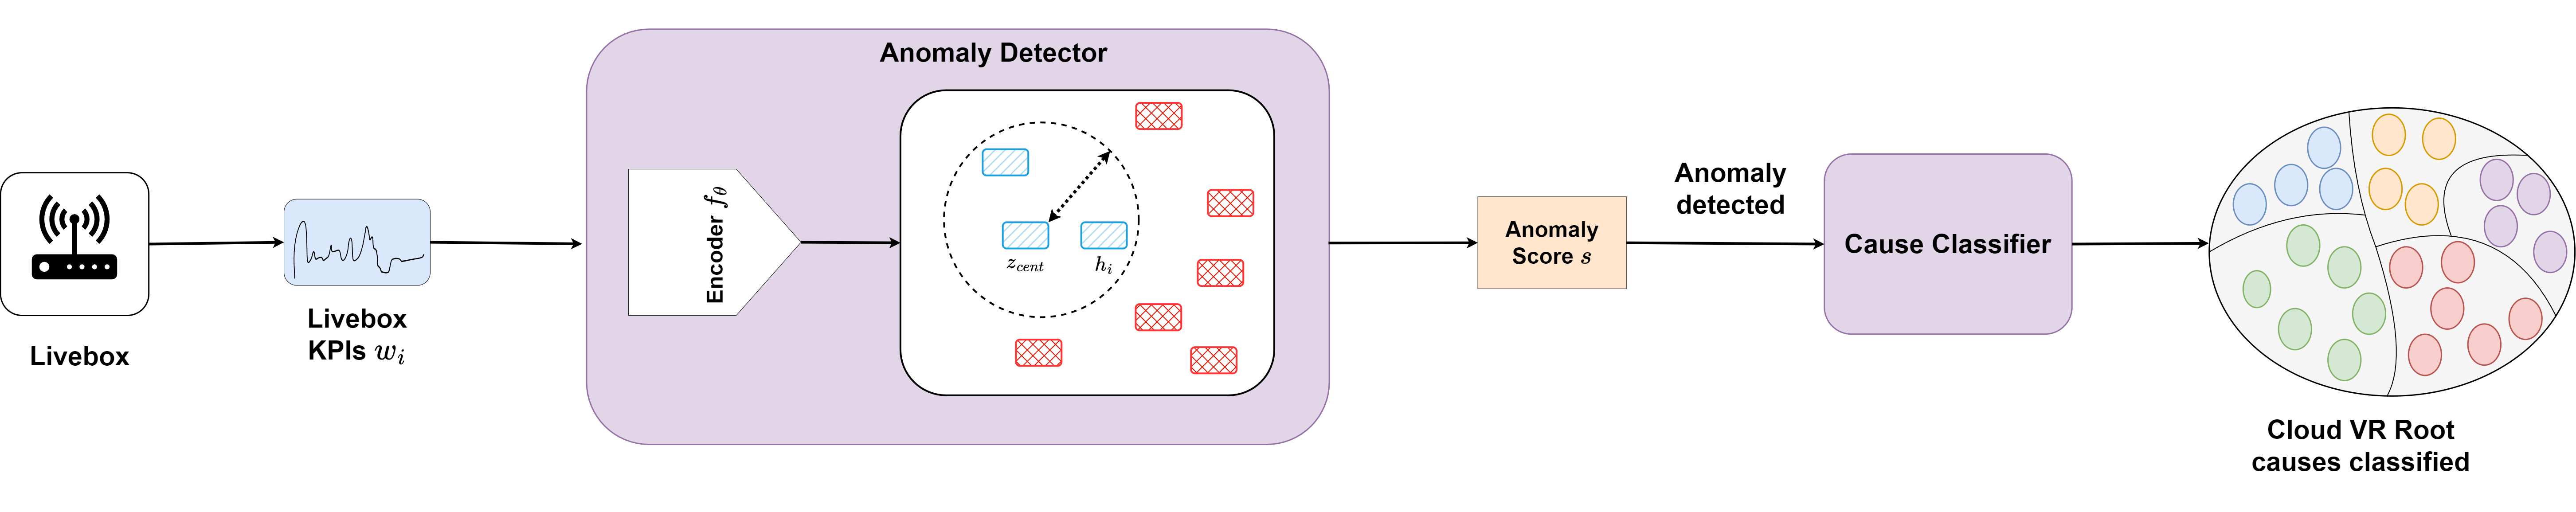
\includegraphics[width=\linewidth]{imgs/chapter_6/diagnostic_rcd.png}
    \caption{RAID framework}
    \label{fig:chap_6:raid}
\end{figure*}

% The rationale behind this choice is motivated by SSL-based classification setups: after learning representations using SSL, the encoder have can discriminate different class so that a shallow classifier trained on top of the representation is sufficient to make predictions.

% The CATS framework's encoder learns discriminative representations that make it easier for a simple classifier to achieve high accuracy. This choice aligns with the principle of leveraging self-supervised representations for downstream supervised tasks.


% \subsection*{Pseudocode for Our Solution}

% \begin{lstlisting}[caption={Anomaly Detection and Root Cause Diagnosis}, label={lst:solution}]
% def train_CATS_model(window_time_series):
%     # Data Augmentation
%     pos_view_1, pos_view_2, neg_view = data_augmentation(window_time_series)
    
%     # Encoding
%     h_pos_1 = encoding(pos_view_1)
%     h_pos_2 = encoding(pos_view_1)
%     h_neg = encoding(pos_view_1)
    
%     # Projection head
%     z_pos_1 = projection(h_pos_1)
%     z_pos_2 = projection(h_pos_2)
%     z_neg = projection(h_neg)
    
%     # Compute the loss function
%     l_gcl = gcl_loss(z_pos_1, z_pos_2, z_neg)
%     l_tcl = tcl_loss(h_pos_1, h_pos_2, h_neg)
    
%     l_total = (l_gcl + l_tcl) / 2
    
%     # Backpropagate
%     l_total.backward()

% def anomaly_detection(data, anomaly_threshold):
%     # Data processing
%     features = preprocess(data)
    
%     # Compute the anomaly score
%     anomaly_score = anomaly_detector(features)
    
%     # Check if the data is anomaly or not
%     if (anomaly_score <= threshold):
%         return normal
%     else: # Anomalies detected => Apply the classifier
%         pred = cause_classifier(features)
%         return pred
    
% \end{lstlisting}

